\chapter{Contribution}

This chapter is divided into multiple sections, which cover the architecture and the expandability of the implementation. The architecture is split into subsections covering the various components that were implemented throughout the thesis. These are the \hyperref[sec:crawler]{Distributed Crawler}, \hyperref[sec:distributed_analysis]{Distributed Analysis}, \hyperref[sec:fronted]{Frontend}, and possible \hyperref[sec:expandability]{Expandability} . Overall it should give the reader an understanding of the motivation and decisions done to implement the requirements.

%Most important chapter of the thesis. Describes what the author contributes as research. Discusses intuition, motivation, describes and reasons about necessity of proposed elements. Defines theses based on reasonable assumptions. Discusses relevant aspects of contribution. Approximately 30 to 40 pages. Can be split into multiple chapters.

\section{Architecture}
\label{sec:architecture}

The architecture covers a database, a data collection, and data analysing unit. It is, in the most classical way, a microservice orientated architecture. Compared to a monolithic application there is a higher focus on single components and their implementation and, therefore, decouple the complexity in its entirety. Another advantage is the scalability, which due to the decoupling allows to run several services of the same type multiple times along each other and increases productivity.

Services themselves can be clustered into the "Distributed Crawler", "Distributed Analysis", "Database", and "Frontend" sections, whereas the database is a third party implementation that is built upon and integrated into the architecture. The visualization of the microservice architecture can be seen in figure \ref{fig:architecture}.

\todo{redo image with clustered sections}
\begin{figure}[H]
    \centering
    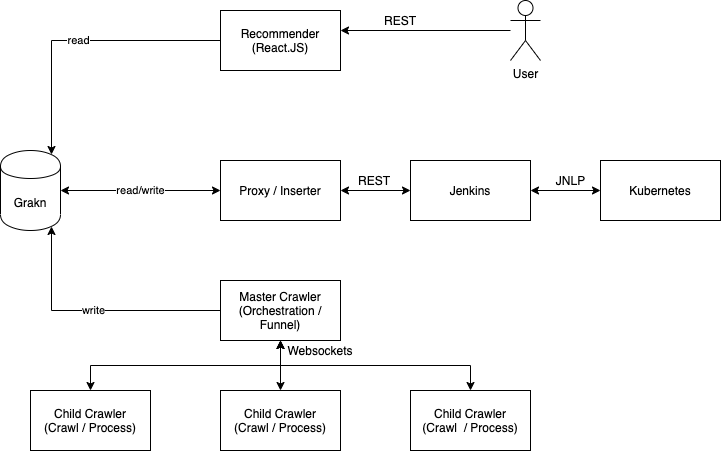
\includegraphics[scale=0.5]{graphics/architecture_v2.png}
    \caption{Architectural representation of the system as a whole}
    \label{fig:architecture}
\end{figure}

\subsection{Database - Grakn.ai}
\label{sec:database}
One of the fundamental decisions is the selection of the database as a lot of other components will have to be built upon it. The creation of a knowledge graph can be done in different ways. One of those is to utilize a graph database, since compared to a NoSQL or SQL database it shows in a clear way the relations between entities. This can be used to build a recommender system due to the sheer amount of data in the graph. The implementation could have been done with a NoSQL or a classical SQL database as well, but would have required more linking of data to represent the same sort of result using a graph database.


One of the biggest graph databases is neo4j\footnote{https://neo4j.com}, which is one of the older ones publicly released in 2007\todo{quote https://neo4j.com/developer/graph-database/\#neo4j-overview}. While neo4j could have been used for the implementation, in direct comparison to grakn, which was released in 2016, the age difference of both projects is visible when it comes to the data representation and their query language "Cypher". Therefore, the graph database Grakn\footnote{https://grakn.ai} was used, which was released in 2016 as mentioned\todo{quote source}.

Grakn describes itself as a knowledge graph engine for the purpose of organizing complex networks of data and making them queryable by performing knowledge engineering\todo{quote https://grakn.ai/grakn-core}. It fully supports the Entity-Relationship model and comes along with a query language called Graql. 

\subsubsection{Entity-Relationship model}
Entity-Relationship models are the de facto standard to represent a schema for a graph database.
\todo{redo er model}
\begin{figure}[H]
    \centering
    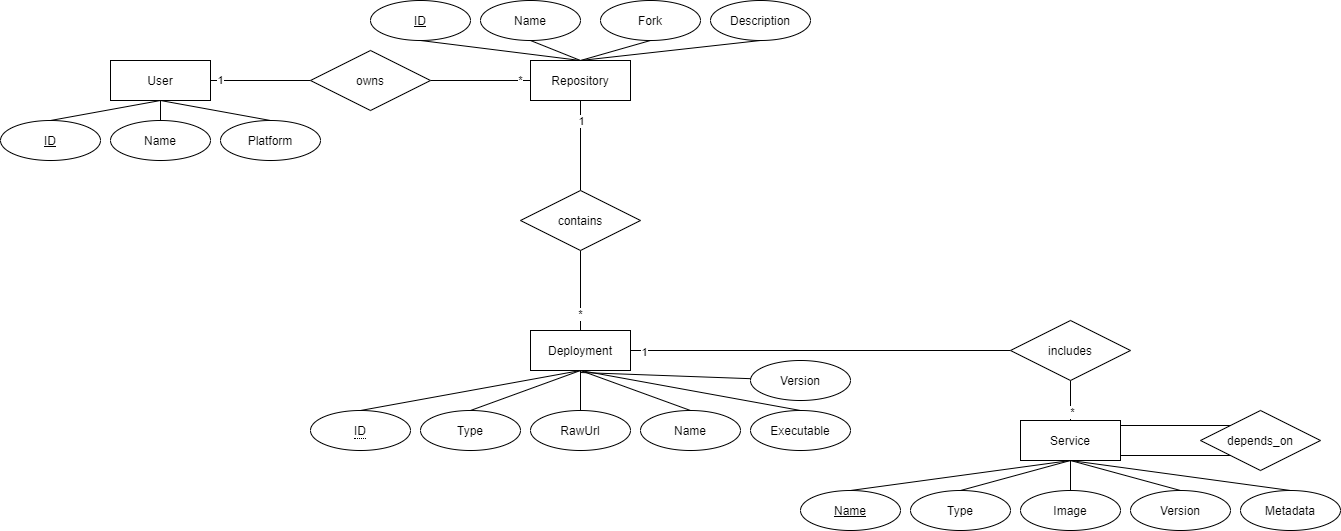
\includegraphics[width=1.2\paperwidth,height=1.2\paperheight,keepaspectratio,angle=270]{graphics/er_database.png}
    \caption{Entity-Relationship model}
    \label{fig:er_model}
\end{figure}

Deployment Scripts do not follow a standard and, therefore, a generalized model has to be created to possibly fit most of them. The focus was lying on the deployment as this entity represents the script itself as a whole. Services that are defined in the deployment script and, thereby, have a direct relationship to the deployment are linked together. In a deployment services can occur unlimited times, however, one service can always only have one deployment. This was kept this way as services, depending on the context, can be differently defined in terms of versions or extra attributes. As one is dealing with a graph database, searching for the best possible fit will still work easy as there is a direct relationship between services and their deployment.
Services can as well depend on themselves, meaning that they are more coupled than others, e.g. a database and a backend, for example. Once more this highly depends on the context and will be further explained in another section in this chapter. \todo{link chapter or explain further}
As the deployment script is usually embedded in a repository, a coupling is taking place there as well. The repository could represent, in a classical way, a repository on either GitHub or Bitbucket, but could also be a website or documentation depending on where it was found. One repository can hold an unlimited amount of deployment scripts and one can possibly belong to multiple repositories. The simple explanation is that the secure hash algorithm is used as key identification and files that have the same content will, therefore, have relationships added to those repositories as well, while still keeping only one deployment entity in the database. This is not used to save storage, but it allows to implicitly draw conclusions from the data. The last entity in the schema is a user that owns unlimited repositories, while one repository can only belong to one user.

One of the favorable aspects of Grakn is how it handles duplicates. As long as one defines unique keys in the attributes of an entity, there will not be a duplicate since those will automatically be dropped on insertion. This will keep the database free from duplicates and allows one to concentrate on the actual implementation of their use case.

The schema is kept general in regards to the domain of different kinds of deployment scripts, while overall favouring the origin from code repositories. A visualization of the schema can be seen in figure \ref{fig:er_model} and gives a basic overview according to current standards in ER models.

Grakn supports the feature of having an attribute as a key attribute and, therefore, provides uniqueness across one entity based on this key. While Grakn provides its own internal ID, it was useful and necessary to give each entity and relation a self defined key attribute to prevent additional mapping of Grakn ID to e.g. GitHub IDs or other elements in order to uniquely identify one relation or entity.

\subsubsection{Open Source Contributions}
\label{sec:opensource}
Grakn is a comparatively new graph database which causes its community to still be rather small. Accordingly, problems that have been solved for other graph databases have yet to be covered for this one. Therefore, some contributions to the project around Grakn and its tools have been covered in the implementation of this thesis.

First of all, Grakn comes along with a tool called "workbase", which essentially is an editor to show and edit the graph that the database contains. This is sufficient for most projects where the graph is rather small. The "workbase" is a Vue/React application wrapped in electron, which is a framework to create desktop applications from JavaScript. Therefore, electron is wrapping the files with chromium and node.js to display the application cross platform. The "workbase" comes along with some flaws as graphs with nodes and edges in the 100.000 area will crash the application due to the limited amount of memory assigned to the chromium process. Even in the area of 10.000 and more, the application starts to stutter under the heavy load.

Therefore, the first contribution in the domain of Grakn is a converter from Grakn to the the Graph Exchange XML Format (GEXF), which is essentially a file format to describe complex networks structures.
The advantage of GEXF is that it is an open specification and, therefore, implemented and used by a variation of applications and tools. One of these tools is Gephi - the open graph viz platform that allows to visualize and analyse networks of sizes in the area of multiple million nodes and edges. Another tool is the NetworkX\footnote{https://networkx.org/} framework for python, which allows to load and write GEXF files and, therefore, analyse networks further in the python universe.

The Grakn to GEXF converter reads a provided Grakn schema and generates proper queries for each entity and relation, followed by querying the database for the results and writing the results to a valid GEXF file. This, in return, can be further used by the tools mentioned earlier. Overall, this will help to further analyse the graph as Grakn itself does not provide any tools for layouting, clustering coefficient, community detection and other metrics that might be interesting to extract out of a graph.

Another open source contribution was done in the direction of cloud compatibility as the open source version of the database does not come along with e.g. a helm chart or, in general, kubernetes manifests to deploy and seed a database one has to build the compatibility themselves. It is important to note that the Grakn database is split between a server and a console (cli) component, which are bundled into one docker image. While this makes it easier to e.g. debug the database it is not suitable to run as a sidecar container in Kubernetes, as one simply does not need the server component for seeding the database. The database can only be seeded if it is running, which makes kubernetes init containers \todo{explain concept in technologies} useless as those will run before the actual container is running. Thereby, a sidecar is needed, meaning an additional container in the same pod to seed the database as soon as the server container is up and running. While this sounds relatively easy, the Grakn console nor the server provide a health route to check whether the database is running. Yes, one can probe the port of the database but this will not guarantee that the database is ready to receive connections. Therefore, the second contribution is a sidecar container, containing a slim alpine image with the Grakn console and a startup script to check for the database for receiving connections and, if needed, seed the database with a schema that can be mounted into the container.
One of the important points of infrastructure as a code is reproducibility, meaning if one runs the code on different systems it should still result in the same end product, thus a manual seeding of the database would not be suitable.

Both contributions are publicly available on GitHub\footnote{https://github.com/Langleu/grakn-to-gexf}\footnote{https://github.com/Langleu/grakn-console}.

\subsection{Distributed Crawler}
\label{sec:crawler}
First and foremost, the main part of the implementation is the so-called "distributed crawler", which follows the master and node pattern, where one entity is the master that controls the spawned nodes. In this thesis, it can also be seen as an orchestrator/information funnel and the crawling/processing unit. The reason for calling it a distributed crawler is that the overall function of this implementation can be seen as a crawler, and distributed in the sense that the nodes can be distributed across multiple data centers.

The implementation was done using Node.js, which is an asynchronous JavaScript runtime that allows to run JavaScript outside of the browser and potentially build scalable applications. One of the big advantages of Node.js is that one can use the synergies of running JavaScript on the server-side and client-side. While this might not be the first thing that comes to mind when thinking about a distributed crawler, it does come in handy as a lot of services offer an API\footnote{Application Programming Interface} that returns JSON\footnote{JavaScript Object Notation} objects. These JSON objects are easier to manage in their native environment compared to other programming languages, where one would rely on a third party implementation and a lot of serialization as the implementation was simply not meant for that specific environment.
As JavaScript runs in a JavaScript engine, the V8 engine developed by Google, it can be extended by creating C++ modules to make certain functions quicker as those would natively run on the system.

The master and crawler nodes are all based on one unified code base. The only difference between the two is the addition of the database connection and the orchestration routes which are both parts of the master node. The default startup parameters for a node are to act as a crawler and connect to the master, which can be changed by setting one environment variable called "TYPE" to "master". The node would, therefore, load the database module, orchestration routes and use the master implementation of the communication channel instead of the node one.
The benefits of a unified code base are that the application could be extended in the future in order to support e.g. leader election or let the master act as a node as well. Depending on the processing power provided, the master could handle, on top of its own capabilities, the ones of a node as well and, therefore, provide more coverage of crawled sources.
Leader election, shortly explained, is that e.g. 4 spawned nodes would elect one of their own to be the master, which often works based on either "first come first serve" basis or other defined constraints.

On a fundamental level, master and node are web servers providing a REST\footnote{Representational State Transfer} API, that allows one to trigger functions either from outside or from the application itself. REST comes along with well-defined methods using "GET", "POST", "DELETE", "PATCH", and some others. In the context of the distributed crawler, the most used methods are "GET" and "POST", as one either wants to receive information or in a sense add information, while "POST" is often used to as well incorporate functions that are not covered by the other methods.
While a REST API grants a good interface for a user or another application, it is not very well suited for bidirectional real-time communication. Since the crawlers are potentially distributed over various data-centers, it can be difficult to keep track of every single one of them, especially for the master as one would need e.g. a domain or another unique identifier to connect to all nodes prior to deploying the master. To counter this issue, another communication channel was introduced - the so-called WebSockets - which allow a real-time bidirectional communication where only the crawler would need to know the unique identifier of the master, instead of the other way around. WebSockets, initially originating from the web browser domain to allow client-server communication, can also be used as a pure client-server communication without a web browser due to Node.js. WebSockets use a TCP socket to communicate through and are on the same OSI layer as HTTP. They make use of topic related channels that client and server have to subscribe to, to be able to send and receive messages about those topics. This bidirectional communication channel will be part of further subsections.

\begin{figure}[H]
    \centering
    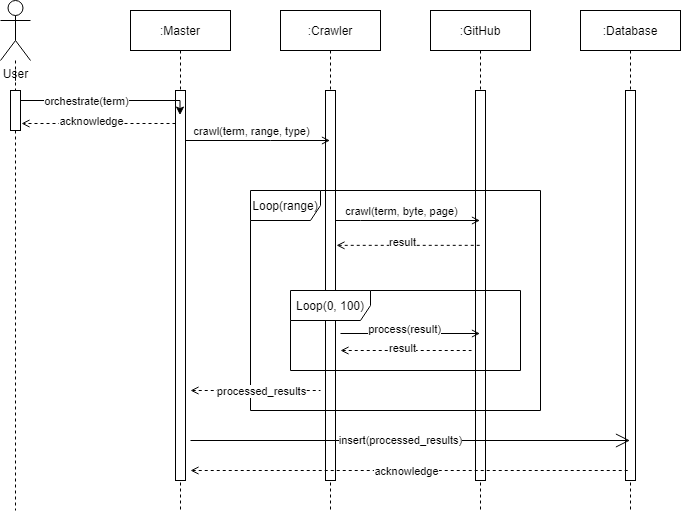
\includegraphics[scale=0.5]{graphics/crawler_sequence.png}
    \caption{Sequence diagram of the Crawler}
    \label{fig:seq_dia_crawler}
\end{figure}

The figure \ref{fig:seq_dia_crawler} visualizes the communication of the distributed crawler as a sequence diagram. The orchestration is initially started with a REST request to the master crawler, which acknowledges the request. The master then sends a request via WebSocket to the crawler with the term to search for, the range it shall cover, and the strategy it shall use. The crawler loops over the range and requests byte by byte and page by page the GitHub API, after a page is covered, it will be processed and the actual file will be requested of GitHub and further analysed. After the processing step, the final results for that particular byte will be send back to the master via WebSocket and then inserted into the database using a gRPC library.

\subsubsection{Information funnel}
\label{sec:informationfunnel}
One of the functions of the master is to act as an information funnel or a proxy to the database. This makes the implementation of the crawler nodes easier as one does not have to worry about connecting to the database and can just use the bidirectional communication channel with the master. From a security point of view, it might also be easier to keep only one communication channel secure compared to multiple small ones, depending on the setup of multiple locations.

Crawlers are essentially preparing and processing what they have crawled within the application and send the finished result to the master, which in return inserts the results into the database. The established bidirectional communication channel will be used, keeping additional overhead small compared to other ways of implementing it.\todo{maybe add http vs sockets, header overhead etc.}

\subsubsection{Orchestration}
\label{sec:orchestration}
As the master and node pattern already suggests, controlling is one of the aspects of a master node. In this case, the job orchestration will be handled from the master node. Therefore, the master provides a REST API that can be consumed by e.g. a user or some sort of automation like cron jobs that trigger crawling based on a schedule. This could have been implemented using WebSockets as well, but a REST API is easier to consume compared to establishing a socket connection and then sending a message for a specific topic.

While orchestration is a REST API route, it utilizes the WebSocket to send messages to its connected nodes and uses those as well for calculating windows that have to be crawled. A window, in this sense, is a range where the crawling should start and end. The orchestrator has a minimum and maximum value in between which should be crawled, which in return is divided by the amount of crawlers that are available at the point of receiving the request for orchestration. Each crawler, therefore, receives a window that should be covered.

\subsubsection{Crawling}
\label{sec:crawling}
The implementation of the crawler makes use of the strategy pattern, which is a behavioral software pattern that allows selecting a strategy/implementation during runtime. This means in particular that there is a generic interface with the defined functions that have to be implemented by each strategy. In Node.js there is no classical object orientation that a lot of people might know from Java. Therefore the implementation makes use of a class that implements the generic interface that then each strategy can extend and implement. Further on there is one main class, which initializes the required strategy during runtime by making use of a switch case.

While this gives one a lot of flexibility and options to further extend this with other strategies it also brings along a couple of negative aspects like having to know which strategies are available and some extra effort into handling the implementation.

The first data source to be crawled and therefore the first strategy was for GitHub. GitHub is the biggest collection of public repositories and ,thereby, offers a good starting point to cover roughly over a million deployment scripts in the case of docker-compose.
GitHub offers an API already in its third iteration with various REST endpoints that return JSON. These can be used for crawling GitHub, which can be done in various ways depending on the information that is required. In case of deployment scripts one would be interested in repositories that house those scripts.
One way to tackle this issue is using a breadth-first search algorithm that traverses through users and their repositories and continues by traversing through their contributors and their respective repositories. Random users could be retrieved by utilizing the GitHub API and the contents of a repository could be analysed by cloning the repository and running a quick find script for a selected deployment script as those usually have a similar naming scheme for the same type of tool. Looking at GitHub as a network graph, this strategy might not find all users that have deployment scripts as not all users have to be connected through one way or another. On top of that one spends a lot of time traversing through users and repositories that are not anyhow related to the topic as in the end deployment scripts are compared to e.g. programming languages etc. a niche topic.

Another way to approach this topic is to utilize a GitHub API that allows one to search through the code of all public repositories and, therefore, be more precise as it will directly return users and repositories related to a topic. This provides the starting point for the GitHub crawler strategy. Since GitHub is quite popular and offers its API for free some of those API routes come with limitations, especially in something so resource-intensive as searching code through all public repositories.
Therefore, the first limitation that GitHub introduced for the "search REST endpoint" is that only authorized users can use this function and with that, the second limitation comes along that requests will be limited to 30 per minute. To circumvent those two limitations each crawler gets assigned a designated GitHub Account with a username and token to authenticate against the API and in case of running into the 30 requests per minute limit the crawler will sleep till the limit is lifted again.
The next limitation is that GitHub will only return a maximum of 1000 results per search query. While this seems difficult to bypass, GitHub brings along the proper tools to do so. One of the query parameters of the "GET" request is simply called "q" and allows one to build complex individual queries that are unique in itself and, therefore, offer up to 1000 results per query. The query parameter "q" can be extended to include the file name and file extension. Deployment scripts are often written in YAML\footnote{YAML Ain't Markup Language} and have come along with the extension ending "yaml" and "yml". Thereby, doubles the number of search results in the case of YAML specific deployment scripts as one can vary between those two different spellings. The most important factor for circumventing the limit of 1000 results is to utilize the size of a file. GitHub allows one to define the size of a file, that one is searching for, in bytes or in a byte range, meaning one could search for all files in a range of 100-102 bytes or in the use case of the thesis to search per byte. This would allow one to create for the same file a unique query every single time.
Of course, GitHub has a limitation for this one as well and only allows to find files up to 384 Kilobyte, which in the context of this thesis is negligible as deployment scripts rarely touch the two-digit Kilobyte area.

Theoretically speaking 384 million files could be covered by just utilizing the size factor without even utilizing such things as extensions, order, or sorting. With those included depending on the type of deployment script, one could easily cover up to a billion search results.

To summarize the GitHub API, it comes along with a lot of limitations but at the same time with all tools needed to circumvent those limitations and, therefore, covering almost all public repositories.

This should give one a perspective as well on why one would utilize a distributed crawler as this allows covering a much wider area and much quicker by spawning more nodes. As previously mentioned in the part about orchestration a window area is defined for crawling, this is limited from 50 bytes to 384 Kilobytes as a 50 byte deployment script will most likely just include the very basics of its potential. One crawler does not cover the full range, except its the only crawler available, but rather the window that was set by the master node.

The following will show an example query of the GitHub code API and its result.
\begin{lstlisting}[language=bash, caption=GitHub Request, breaklines=true, label=lst:github_request, numbers=left,  basicstyle=\footnotesize\singlespacing]
curl --location --request GET 'https://api.github.com/search/code?q=filename:docker-compose.yml+size=1234&page=1&per_page=100&order=asc&sort=indexed' \
--header 'Authorization: token $token'
\end{lstlisting}
\begin{lstlisting}[caption=GitHub Response, breaklines=true, label=lst:github_response, numbers=left,  basicstyle=\footnotesize\singlespacing]
{
    "total_count": 213,
    "incomplete_results": true,
    "items": [
        {
            "name": "docker-compose.yml",
            "path": "docker/docker-compose.yml",
            "sha": "2a4ee33f9c924e2a107160e4cbbeac17fa8525f9",
            "url": "https://api.github.com/repositories/000000001/contents/docker/docker-compose.yml?ref=f657460284d463a2792f35f50728c74b9a52504e",
            "git_url": "https://api.github.com/repositories/000000001/git/blobs/2a4ee33f9c924e2a107160e4cbbeac17fa8525f9",
            "html_url": "https://github.com/username/repository/blob/f657460284d463a2792f35f50728c74b9a52504e/docker/docker-compose.yml",
            "repository": {
                "id": 000000001,
                "node_id": "PDCwOlJlcC9zaXRvcnkxMzU3MjI5OTk=",
                "name": "repository",
                "full_name": "username/repository",
                "private": false,
                "owner": {
                    "login": "username",
                    "id": 0000001,
                    "node_id": "MDQ6MEClcjYwNzY5MTE=",
                    "avatar_url": "https://avatars0.githubusercontent.com/u/0000001?v=4",
                    "gravatar_id": "",
                    "url": "https://api.github.com/users/username",
                    "html_url": "https://github.com/username",
                    ...
                    "type": "User",
                    "site_admin": false
                },
                "html_url": "https://github.com/username/repository",
                "description": "simple description",
                "fork": false,
                ...
            },
            "score": 1.0
        },
        ...
    ]
}
\end{lstlisting}

All user related data was redacted from both listings in \ref{lst:github_request} and \ref{lst:github_response}.
The code in listing \ref{lst:github_request} shows an example request for the GitHub code API searching for "docker-compose.yml" files with the bytes 1234.
Listing \ref{lst:github_response} shows the response for of the request in the JSON format. It shows a total count of 213 files for the bytes 1234 and incomplete results as well, this means that there are likely more results, but the request ran into a timeout and returned all possible found items with a limit of 100. The user object contains additional direct links for each imaginable topic surrounding a user, e.g. direct links to followers, following, starred, repositories, and much more. The same happens in the repository object with direct links to forks, contributors, issues, and more. Each object in the items array has a score as well, which is nowhere described in the GitHub API documentation, but always results to 1.0 in all found items.
Overall the response includes all necessary information to further process the data in the processing step.

\subsubsection{Processing}
\label{sec:processing}
Processing was built similar to crawling, meaning it is based on a strategy pattern to be as flexible as possible and gives a certain extensibility for future projects. As it is based on the strategy pattern it comes along with the same advantages and disadvantages as already described in the section about the crawler.
While the crawling itself only covers the points of collecting data, the processing step is the predecessor to inserting the data into the database, but the collected data has to be first brought into alignment with the database schema, earlier described in the section about Grakn.

For this the processing step fetches the deployment script, or uses an already provided script, and parses the script with a YAML parser, as most deployment scripts are defined in this structure, and creates arrays of entities and relations necessary to satisfy the database schema. This YAML parser will automatically discard all deployment scripts that could not be parsed as those would also not be able to be parsed by the final product, e.g. docker-compose. Therefore, all data in the database are syntactically correct and can be further used by e.g. docker-compose or depending on the strategy the tool that was kept in mind for it.

In the case of docker-compose, the script will be parsed and split into the entities of services and deployment. For relations it will be parsed into includes and depends\_on, where includes is the general relation between a service and deployment and depends\_on describes the possible dependency of a service to another service, e.g. dependency of database and application.

After completely processing the deployment script and general information about the origin the processed data is sent to the server component or informational tunnel using the bidirectional channel of the WebSocket.

\subsubsection{Data insertion}
\label{sec:data_insertion}
After successfully collecting and processing the data, the last step is to insert the data into the database. For this step, each entity and relation has its own template, which in the end results in one query for inserting the selected type. This template system is built on a similar thought as the strategy patterns, as a template simply resembles a strategy for a certain provided type. The information funnel, therefore, iterates through each array and selects the proper type to then insert the data.
Grakn is built in a way to first create a database connection, followed by a session, followed by a transaction for either reading or writing and as the last step one has to close the transaction again to commit the actual data or to properly close the reading transaction.
Each connection will use a certain amount of memory to keep the connection alive and each insertion will come along with a certain amount of processing power as everything has to be linked in the graph.
The writing transaction can contain an unlimited amount of queries to insert, but one has to be careful as duplicates will cause the write transaction to fail as a whole, meaning that data that might be unknown will not be written to the actual database. Thereby, for this implementation, each query was treated as a single write transaction to circumvent possible data loss. This was done as a user can have an unlimited amount of repositories and, therefore, possibly deployments. A deployment can also be used by different users in different repositories and, thereby, have an already known entity in the database. It is important to collect as much data as possible as deployments that are contained in multiple repositories might be of greater importance than deployment scripts that are unique, but this will be covered in the evaluation chapter.

The initial database connection and session creation don't have a time constraint or are important for actual data commitment, but in case of failure, a new session will be created as it can't be verified that the current session is still valid.

\begin{lstlisting}[caption=Process response, breaklines=true, label=lst:process_response, numbers=left,  basicstyle=\footnotesize\singlespacing]
[
    {
        "user": {
            "id": "00001",
            "name": "username",
            "platform": "github"
        },
        "repository": {
            "id": "00002",
            "name": "repository",
            "description": "simple description",
            "fork": false
        },
        "deployment": {
            "rawUrl": "https://raw.githubusercontent.com/username/repository/...",
            "type": "docker-compose",
            "name": "docker-compose.yml",
            "id": "SHA-Hash-deployment",
            "executable": -1, // not yet evaluated
            "score": -1, // not yet evaluated
            "version": "3" // docker-compose version
        },
        "services": [
            {
                "rid": "SHA-Hash-nginx", // uses service name and deployment id
                "name": "reverse-proxy",
                "type": "Docker",
                "image": "nginx",
                "version": "alpine",
                "metadata": "{ports: 80, environment: EXAMPLE=EXAMPLE, command: nginx}"
            },
            {
                "rid": "SHA-Hash-node", // uses service name and deployment id
                "name": "frontend",
                "type": "Docker",
                "image": "node",
                "version": "alpine",
                "metadata": "{ports: 8080, environment: EXAMPLE=EXAMPLE, command: node index.js}"
            }
        ],
        "depends_on": [
            {
                "serviceA": "SHA-Hash-node",
                "serviceB": "SHA-Hash-nginx"
            }
        ],
        "includes": [
            {
                "deploymentId": "SHA-Hash-deployment",
                "serviceId": "SHA-Hash-nginx"
            },
            {
                "deploymentId": "SHA-Hash-deployment",
                "serviceId": "SHA-Hash-node"
            }
        ],
        "owns": [
            {
                "userId": "00001",
                "repoId": "00002"
            }
        ],
        "contains": [
            {
                "repoId": "00002",
                "deploymentId": "SHA-Hash-deployment"
            }
        ]
    }
]
\end{lstlisting}

An example YAML is described in the listing \ref{lst:process_response} and consists of several objects and arrays. There is the user, repository, and deployment object, that all describe data, which were crawled via the GitHub API and can be seen in listing \ref{lst:github_response}.
The Array services describes each service node, parsed from the "docker-compose" file. Depends\_on, includes, owns, and contains are all edge related arrays and contain the data about which node is connected to which other node.
This data is further used to generate each individual query for inserting into the database. An example query for the user can be seen in the listing \ref{lst:grakn_query} and works similarly for the other entities as well, by creating a query string containing all values according to the database schema.

\begin{lstlisting}[caption=Grakn query, breaklines=true, label=lst:grakn_query, numbers=left,  basicstyle=\footnotesize\singlespacing]
insert $user isa user, has rid "00001", has name "username", has platform "github", has schemaVersion 1, has updated Date, has created Date;
\end{lstlisting}

\subsection{Distributed Analysis}
\label{sec:distributed_analysis}
To further analyse the data a system was required that could potentially deal with a lot of data but at the same time not interfere with any running processes. A distributed system that could scale horizontally similar to the concept of the crawler could further complement the whole system. This once more would be a microservice itself and decoupled from the rest of the architecture, meaning possible flexibility in the choice of tooling and implementation. Therefore, this section will deal with the choice of tooling, different possible tools, vulnerability scanning, calculation of a score, which will further be used for the recommendation system, and isolation.

\subsubsection{Choice of Tooling}
\label{sec:choice_of_tooling}
To determine the final choice of tooling for the task of a distributed analysis one has to consider what has to be achieved, how flexible it is, and whether it can be extended in the future. Time is not too much of importance in this part as due to possible horizontal scaling this can be complemented by simply running it on more machines.

The task that had to be solved was to run a linear task of executing the deployment script, and, thereby, determining whether the deployment script is executable or not, followed by a vulnerability scan to determine a security factor, checking the deployment script for best practices and in the end calculates the final score, which is sent back to an API that updates the database.

The first iteration brought forward a couple of possible candidates. One of those is the possibility of using a Continuous Integration (CI) system, which is known for running a lot of tests parallel, which can, depending on the CI, be extended with the usage of plugins and is quite flexible and extendable. Another option was to create a REST API that runs certain predefined steps on the provided data. The last option was to use a workflow engine, which is more known in the area of business processes, but in the end, all of it is a rather linear process, which could also be done by such an engine.

All of those options bring along some positive and negative aspects and all of them would be capable of further analysing the data and calculating a score based on the flow earlier described.

Starting off with the option of creating a REST API and processor for doing those simple steps. While this gives one a lot of flexibility and expandability, it will at some point run into the problem of properly isolating the process that is executed by running the deployment script. As this thesis mainly focuses on the aspects of docker images, which are in itself already an isolation, it will at some point encounter problems with possible port mappings from local ports to remote ports or mounting and using of the same files or folders. To fix this issue one could wrap the REST API into a docker container itself and run it in Kubernetes, while this would diminish the issues it would arise new ones. Suddenly routing would become a problem as one would have to spawn a new endpoint for each analysis one wants to run, which in return would mean that either another component is necessary to make sure that only one REST API receives one data package and, therefore, having another master - node pattern.
This option was dismissed as the problem has been solved by a lot of other people already in the form of either a workflow engine or a CI system.

Using a workflow engine would already solve the problem of running a certain process in order, but at the same time introduce new issues as workflow engines, in general, come along with an extra component that monitors and manages the processes, hence the engine. They are not made to transport a lot of data between workers and, thereby, require an extra database to partly save data in there to transfer information from one worker to another. For the concept of isolation, a workflow engine would exist and have workers spawned that all deal with certain steps, but this does introduce another problem at the same time as one might not know prior how many workers of each task type are needed as some tasks are quicker than others and also introduce the overhead of having to clean up the workspace to have a neutral ground for each task execution. While a workflow engine is certainly an option to solve this task the lack of proper scaling and the additional need to keep the workspace clean dismissed this option as well.

The last option was to use a continuous integration tool, which exists in a broad spectrum from SaaS (Software as a Service) tools to self-hosted tools, from open source editions to enterprise editions. In the end, most of the currently existing CI tools solve the same problem in a similar fashion. The option of using SaaS was not really possible as the tool would not be used in the way it was intended to be used, as unknown code should be covered. The test has to be as general as possible and SaaS tools usually require one to create a file or reference in the code repository of a project to confirm actual ownership of the code and at the same time provide the tasks or tests that should be run.
For the purpose of the thesis, Jenkins was used, which described itself as an open-source automation server\todo{insert https://jenkins.io reference} and is often used in the area of continuous integration and continuous delivery. It is known for being extendable due to the sheer amount of plugins that exist for it as its first stable release was in 2010. Jenkins is essentially a CI/CD tool, but at the same time can be extended to run any process that one would want to execute and, thereby, was from a technical point of view a good choice for this project.

\subsubsection{Importance of Isolation}
\label{sec:importance_of_isolation}
To further explain the choice of Jenkins one has to think about isolation. The payload that is being executed is unknown as any deployment script was written by a third party. If talking about e.g. docker-compose the damage that can be done by executing it is rather slim, since one would have to break out of the container itself, but as the project can be extended by other possible candidates it's good to find a solution that fits possible future extensions as well. On the other hand, docker-compose can build local images as well that could possibly copy files from the system and later on use them in a malicious way by uploading them to an attacker's storage. Thus, it is important to use an extra layer of isolation.

Jenkins, with the use of plugins, supports a multitude of options to run pipelines in different environments.
Possible options are to execute those pipelines on the Jenkins instance itself, which if it is hosted in the right environment could be enough already, but at the same time, it would contradict the requirement of scaling it horizontally as the instance would be limited to the resources it is assigned to or the resources of where it's running in. While it's possible to have multiple Jenkins instances running and control them with a proxy in front of it to route traffic to A or B depending on the workload of one instance, it is not a best practice and rarely seen in an actual working environment except for fault tolerance.

Another way to achieve isolation and horizontal scaling is to deploy so-called Jenkins agents to dedicated machines with the sole purpose of executing Jobs, which in the sense of Jenkins is the execution of a pipeline. While this is a better option than executing pipelines directly on the master instance it still comes along with limitations as one needs to set up the agents manually and configure them to talk to the master instance. For the communication, there are different protocols that can be used, which are WebSockets, JNLP, or the usage of Kafka via a plugin. WebSockets are still in beta stage\footnote{https://github.com/jenkinsci/remoting/blob/master/docs/protocols.md} and not widely used, same as the Kafka plugin, which is not in beta anymore but simply not as widespread as JNLP. JNLP is the Java Web Start protocol and makes use of a TCP connection in the end.

Coming to the cloud era, tools like Docker and Kubernetes gained a lot of traction and while Jenkins was built in an era prior to that the possibility of plugins enables Jenkins to fully exhaust the possibilities of the cloud.
Mounting the Docker socket directly into Jenkins, which enables Jenkins to directly talk to Docker and run pipeline steps in a predefined container is one possibility, but limits Jenkins to the local resources and is not compatible with scalability and proper isolation as the Docker socket is shared. Containers binding to local ports would possibly break it for other running pipelines. To stay within Docker one could utilize Docker Swarm to spawn agents that communicate back to the main Jenkins using the JNLP protocol. While this is a valid option it comes with some limitations as it overcomplicates the pipeline due to the requirement of starting each extra required tool manually using "docker start" and "docker exec" to interact with it.

Kubernetes on the other hand provides proper isolation and allows to scale horizontally only limited by the number of nodes provided. The concept of pods allows the structuring of pipelines in an easier way compared to Docker Swarm. A pod is a collection of containers that all share network and storage, which in the context of Kubernetes make it easier to interact with. E.g. a pod has a Docker in Docker container to provide a Docker socket to run e.g. docker-compose files, a container running the vulnerability scan tool, and another container running Ubuntu or Alpine for additional tooling. In the end, the pod always houses a JNLP inbound agent as well to create the connection to the Jenkins master. Compared to Docker Swarm one does not have to start each required container individually but all of them are started and ready to use from the beginning of the pipeline and the shared network and storage make it easier to interact with files and services from different containers whenever needed.
Further on to complement Jenkins the option of Kubernetes was used to use a cluster to execute all running pipelines.

\todo{possible limitations of Kubernetes? Possibly coverered in Technologies}
\subsubsection{Vulnerability Scanning}
\label{sec:vulnerability_scanning}
To define a score it might be of interest how vulnerable a docker image is. A docker image is essentially a snapshot of a subset of an operating system, meaning that any vulnerability that wasn't fixed at this point in time will still exist in the image till it's rebuilt without the usage of a cache as often Docker just reuses layers if not otherwise instructed. The same can be said for any programming language running inside it e.g. Java, NodeJS, or Python.

For this purpose one can make use of vulnerability scanning tools, where currently three popular options exist, those being Anchore Engine, Clair, and Trivy. \todo{add footnotes for each tool}
All of them solve the issue of scanning images in different ways, all of them utilize a database filled with vulnerabilities called CVE (Common Vulnerabilities and Exposures). CVE is a standardized list of vulnerabilities, which makes exchanging and reporting them easier.
In the end, all three scanners have different accuracies for detecting vulnerabilities with no clear winner when comparing them using the same images. See figure \ref{fig:docker_comparison} for comparison. \todo{explain figure further}

\todo{add source https://www.a10o.net/devsecops/docker-image-security-static-analysis-tool-comparison-anchore-engine-vs-clair-vs-trivy/}
\begin{figure}[H]
    \centering
    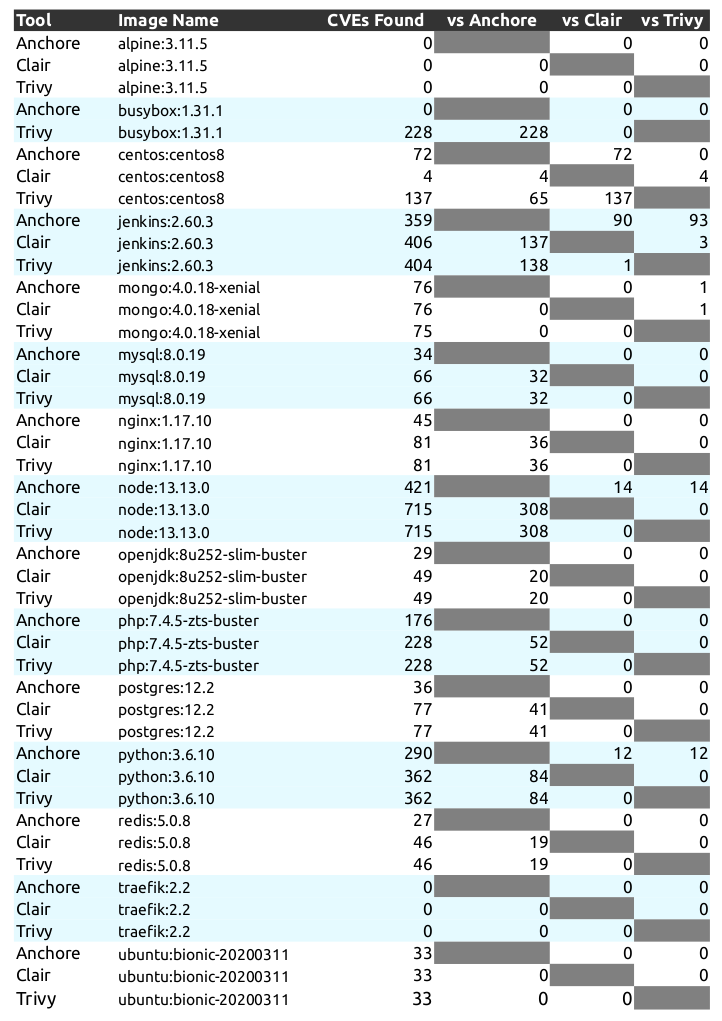
\includegraphics[scale=0.5]{graphics/Docker-Image-Static-Analysis-Tool-Comparison-Table.png}
    \caption{Comparison of Anchore Engine, Clair, and Trivy}
    \label{fig:docker_comparison}
\end{figure}

Some of the tools are easier to implement than others for the purpose of e.g. continuous integration, which is more or less the case for this thesis. Anchore Engine and Clair have to be deployed as a service and need to be accessible for the pipeline. In the case of Kubernetes, this isn't an issue, but it comes along with additional overhead as those tools were simply not developed as a target of CI. Anchore Engine in this case is better than Clair as it comes along with a ready to use CLI\footnote{Command Line Interface}, while Clair requires one to use a third party implementation to interact with it. Trivy was built for the purpose of CI and can be integrated as another container in the Kubernetes pod, which then pulls the latest database filled with CVEs and runs the scan against the defined images in the pipeline, e.g. locally built images or images pulled from Docker registries. \todo{further go into detail how they work}

Trivy was selected due to its easier implementation and amount of output it delivers when detecting vulnerabilities, as those can be further used for calculating a score. First of all, it delivers IDs, names, and descriptions of a vulnerability and more important the severity, which is categorized in critical, high, medium, low, and unknown. While this is already a good indication of how severe a vulnerability is, Trivy delivers additional metrics as well according to the CVSS\footnote{Common Vulnerability Scoring System}, which is an industry-standard for scoring vulnerabilities. The CVSS is divided into three metric groups, which are base, temporal, and environmental, each consisting of further metrics to determine a final score \todo{reference https://www.first.org/cvss/v3.1/specification-document}.
From those metrics, some interesting are e.g. the Attack Vector (AV), which describes how possible the exploitation of a vulnerability is, or the User Interaction (UI), whether another user is required besides the attacker for the exploitation to succeed. Besides that, there are many more metrics that are evaluated to determine a final score and can be read up in the official specification provided by the FIRST.Org, which hosts the CVSS special interest group that is already working on the next version of the specification.
Finally, the CVSS score is divided into numerical ranges to determine the severity, which can be seen in table \ref{cvss_table}.
\begin{table}[h!]
    \centering
    \begin{tabular}{ |c|c| }
    \hline
    Severity & Base Score Range \\
    \hline
         None & 0.0 \\
         Low & 0.1-3.9\\
         Medium & 4.0-6.9\\
         High & 7.0-8.9\\
         Critical & 9.0 - 10.0\\
    \hline
    \end{tabular}
    \caption{CVSS v3.0 Ratings}
    \label{cvss_table}
\end{table}

As the CVSS is an open specification it can be used by anyone. Different organizations have the goal of providing a database with a CVSS score for each identified vulnerability. These organizations are in particular Red Hat and the NIST\footnote{National Institute of Standards and Technology}. Scores from both databases can differ, as metrics can be evaluated differently by different organizations, therefore for the consistency of this thesis the database of the NIST was chosen due to the overall amount of rated vulnerabilities compared to the one provided by Red Hat.
\subsubsection{Calculation of Score}
\label{sec:calculation_of_score}
For the calculation of a score, one has to take a look at all the steps that would be executed by the pipeline. Some of those steps were already described in detail e.g. vulnerability scanning but others like best practices or execution of the deployment script were only briefly mentioned.

The execution of the deployment script shall determine whether the script can be run at all or not, this metric shall help how useful the script might be for usage as a non-executable script might need extra data or images, which are not accessible to the public and thereby of less interest to one. For this, the Docker socket, in the Kubernetes pod of the agent, is directly used to execute the script and afterwards check all containers whether they are either running or exited with a code other than successful. Either result will be set as an environment variable in the pipeline and used later on.

Next on the file length is determined as the longer the file the more the file might be of interest to a reader, as it contains more information compared to a basic script.

For determining whether best practices were followed a tool called Conftest is used, which is published by the Open Policy Agent project under the organization of the Cloud Native Computing Foundation. Conftest enables developers to test their structured configuration data \todo{reference https://github.com/open-policy-agent/conftest }, which YAML is considered as well.
These best practices are opinionated best practices defined by the author and kept general as docker-compose in itself is kept simple. Following best practices are checked for in case of docker-compose: \\
\begin{itemize}
    \item images should be pinned, meaning the latest tag should not be used
    \item images should have a tag as otherwise latest is used implicitly
    \item the compose file should state a version
    \item a build should state an image, which docker automatically uses for tagging
    \item dependencies should be set if a database is involved
    \item if a network is defined then the global networks should be set as well
    \item if a volume is defined then the global volumes should be set as well
\end{itemize}

Conftest checks against these predefined rules and returns the number of tests failed and passed, which can be further used to extract a numerical value.

The step of vulnerabilities scans was already covered in detail, but there is a difference between scripts that were executable and those not. The following is another point why Trivy was used as it allows to scan local images and remote images. In the case of non-executable scripts, the images used are being parsed from the script and then analysed by Trivy, as those images will likely not exist in the local context. For scripts that are executable, the image is derived from the list of all containers that are either running or have run. This covers all locally build images as well. Those are saved locally through docker as an archive and can be further analysed by Trivy. This would not be possible in the case of Clair or Anchore Engine as the actual analysis is run remotely.

As the last step, the score is calculated by using normalization. Each of the previous steps resulted in a numerical value one way or another. Four values exist of different importance. Thereby, both the vulnerability score and the best practices score are given a 1/3 of the total score. It is important to know whether a file is executable or not, but at the same time, the script still brings valuable information and is, thereby, given 1/6 of the total score. The file length is given a 1/6 as well as the longer the better but at the same time there is a limit of a maximum of 300 lines, as anything above this value is most likely not bringing any value, as said before docker-compose is a rather simple system that does not have too much complexity to justify such a long file.
All values were normalized in the range of 0 to 10 and afterwards scaled according to their percentage of the total score. For this, the min-max normalization was used, since all of the values had predefined lower and upper limits. While a Z-score normalization would be preferable there was no historic data that could have been utilized.
\todo{this could be something that could be done in the future based on the current data --> evaluation}

Other values that were considered that could be tested for but left out were startup time and choice of the docker registry.
The startup time was not a metric that could be anyhow justified to be free of interference. There are a lot of factors that can change this value even if the same script is run multiple times. E.g. current workload of the node that the pod is running on and, thereby, possibly less available resources compared to a previous run. One may argue that resource limits should be set for the Jenkins agents, but as the payload that is running is completely unknown at startup time it could possibly interfere with the successful execution of some scripts. On top of that a network interference can happen as well in case a container is pulled slower from the registry or the building of an image takes longer due to a low download speed. Therefore, the time it takes to execute a script was left out as a lot of factors play into it.

The choice of registry was an acceptable point till the introduction of vulnerability scans as a step into the pipeline, since some registries scan their pushed images by default for vulnerabilities. This registry, in particular, is Quay\footnote{https://quay.io}, but at the same time, Docker's own registry and Google offer this service as well if enabled. Thereby, all registries are considered equal in the sense of feature parity. Overall there has been quite a shift in the area of Docker registries recently, but this will be covered further in the evaluation. \todo{Dockers monetization strategy and amazons newly announced registry} \todo{possible last time that something like this can happen as docker will soon switch over to deleting old images that are not used anymore}

Overall the score is a numerical value between 0 and 100 and can further on be used for the recommender system.

\subsubsection{Orchestrator / Funnel}
\label{sec:proxy}
Similar to the already described orchestrator and information funnel in the distributed crawler, a control unit was needed as well for the distributed analysis. This would orchestrate new jobs for Jenkins and update the database with the scores returned from those jobs. This orchestrator consists of a simply REST API, an inserter, and a queue.

The REST API consists of two routes. One has the purpose of updating the entry in the database with the new values in case of a successful run and the other one has the purpose of removing failed builds from the queue to free it up for new job runs.

The queue is a simple singleton that keeps track of two arrays for database entries that need to be processed and entries that are currently being processed. Its main functions are to return a random object from the to be processed queue and to keep this exact queue free from duplicates as the database will return the same objects for the same query and, thereby, duplicates are removed at the application level.

For orchestrating new jobs the inserter will run certain functions based on a temporal value. Every 30 seconds the database will be queried for yet unprocessed entries till it houses a predefined maximum value of 100 entries. Every 2 seconds the length of the process queue is checked and depending on a predefined value a REST request is sent to Jenkins to schedule a new job with the required parameters to run the job. This predefined value is set to 20 and can be changed depending on the setup as it highly depends on the Kubernetes cluster. For the purpose of this thesis, it was set to 20 as it seemed the most stable in the provided environment.

The orchestrator acts as a proxy between Jenkins and the database for reasons of reliability and abstraction purposes.
An implementation could have been done without the necessity of an additional proxy by extending the Jenkins pipelines with two simple steps. The first step would utilize an additional container with e.g. Node.js to run the Grakn.ai library to query for database entries. This would be followed by the steps explained earlier in the part about the calculation of the score and finished by another step to update the values in the database for the previously queried entry. This would likely be not as efficient due to querying the database for a single entry, which would result in the same entry for each pipeline till the entry is updated with new values, thereby, running the pipeline 20 times at the same time would result in 20 pipelines running the tests for the same values. The reason being that the database simply caches queries that are not unique for quicker responses. A proxy was implemented to take care of scheduling jobs, updating the database and keeping duplicates out of the system. Being its own microservice the implementation could have been done in any language but was done with similar frameworks as the information funnel.
\subsection{Frontend}
\label{sec:fronted}
For the graphical user interface of the recommender system, the language of JavaScript and its frameworks were used once more. While everything is a microservice in itself already and thereby decoupled from the other services, the implementation can be done in any language, but the synergies of using the same language for everything were used due to the prior knowledge and background in the Node.js framework.
The frontend could have been written in pure JavaScript, HTML, and CSS, but for the purpose of this thesis, a frontend framework was utilized. It gives one a certain abstraction compared to doing everything in its pure form and allows one to write everything in JavaScript. There are plenty of frontend frameworks to choose from with similar popularity and use cases, in the end, it comes down to preference as the job could be done in any of those. Due to prior knowledge in this topic, there were two candidates to choose from, which are React and Vue.js.

React was developed in 2013 by Facebook\todo{add reference} and offers a modular system, meaning one develops modules that bundle logic and presentation in one object. This allows the exchange of those modules across different projects and rapidly increases the development of new applications as a lot of problems have already been solved and published by someone else.

Vue.js was developed in 2014 and published by Evan You\todo{add reference}. In its scope, it's the same as React and only differs in nuances. One of these is the point of easier acquiring the knowledge to properly master the framework, but on the other hand, lacks in regards to publicly available modules. In comparison, the community of React is much bigger and, therefore, provides more modules even for topics that are niche and have a small community in the first place. The difference of the community size and popularity can simply be explained by having such a big company like Facebook as a project maintainer.

Due to the support of some niche modules, the framework of React was selected.

While React is a framework itself a lot of frameworks building up on React have emerged that all deal with different problems. React in itself is a pure frontend framework and has no out of the box support for a backend, which is still needed to interact with the database and deliver the initial application. Thus, the Next.js framework was selected as it complements React by offering a simple out of the box solution for creating a REST API.

The recommender system offers an input field to type in the image or images one is looking for and a drop-down menu that offers all available types of deployment scripts. The inputs are sent to the recommendation API, which in return queries the database for 10 deployment scripts with the highest score that offer all typed in images. If no such script exists then it tries to find deployment scripts for each image individually. The returned entries build a selectable table in the frontend, which if clicked on sends another API request to fetch all services and its connections related to the selected deployment script to in return visualize the deployment script as a graph of all connected services.

Overall the frontend is kept simple to offer the user a self-explanatory user experience and allowing to quickly find related deployment scripts that can be used as inspiration for ones own script. Therefore, the type of recommender system is a content-based recommender system as all scores are precomputed based on the implementation of the scoring explained prior.
\section{Expandability}
\label{sec:expandability}
The focus of the thesis was on deployment scripts related to docker-compose, but one of the aims of this contribution was to implement everything as expandable as possible.
Starting with the database the entity-relationship model was created as generic as possible with options to extend it to a different type of sources and deployment scripts by offering the type parameter, which make it easier to select certain types while querying. On the other hand, the database can be extended as well by creating new keyspaces related to different types of deployment scripts. These could utilize the same schema, but would probably benefit from being decoupled from other deployment scripts in terms of performance as not a single graph with all information has to be kept but rather graphs related to the same type.

During the chapter about the distributed crawler (\ref{sec:crawler}), the strategy pattern was already introduced, which offers the development of strategy in terms of crawling sources and processing.
For crawling it could be extended to different code repositories like Bitbucket, GitLab and privately hosted repositories. On top of that even such things as search engines could be utilized as those crawl most of the internet already and offer indexed lists, which could offer a similar efficiency as the GitHub code API. The search term for all crawling strategies is variable, meaning it can be used for any type of deployment script as long as it has a similar naming scheme e.g. Kustomize in case of Kubernetes. Strategies for other deployment scripts could be developed as well, which don't follow a naming scheme e.g. Helm, which offers a registry for their so-called charts. For something like Ansible it might be a bit more difficult as it doesn't offer a common filename nor a unique identifier in the script, but even for Ansible GitHub offers eighty thousand unique files called "playbook.yml" and custom strategies could be built that utilize other methods to find Ansible scripts. The table \ref{deployment_script_occurrences} shows approximately the amount of related deployment scripts of some tools on GitHub. An exact number can not be given due to the GitHub API experiencing a timeout after a certain time and returning all results it collected till then.

\begin{table}[h!]
    \centering
    \begin{tabular}{ |c|c| }
    \hline
    Type & Occurrences \\
    \hline
         Docker-Compose & > 1.260.580 \\
         Vagrant & > 256.348\\
         Ansible & > 121,388\\
         Kustomize & > 65.481\\
         Helm & 2061*\\
    \hline
    \end{tabular}
    \caption{Approximately found deployment scripts on GitHub. * Helm artifact repository}
    \label{deployment_script_occurrences}
\end{table}

The processing of those deployment scripts supports the strategy pattern as well and a strategy has to be developed for each deployment script that one would want to insert into the database as each type of deployment script is unique and has to be altered to the database scheme.

For the distributed analysis the underlying layer of Jenkins and Kubernetes can be used as well and only a new job has to be developed, which could consist of similar tasks compared to the docker-compose pipeline. The deployment script could be executed in an isolated environment, some best practices could be tested with the help of Conftest, vulnerabilities could be scanned as well for defined images in those deployment scripts and the file size could be utilized as a metric as well. Overall the currently defined pipeline could act as a very good starting point for other types of deployment scripts. In case of Kustomize and Helm, the docker in docker container could be switched for a kubernetes in docker container, which allows testing Kubernetes related scripts in a continuous integration environment.

For the proxy, an additional instance could be spawned that is configured by providing environment variables with all related information to trigger the proper pipeline and query the required entries. It's simpler to spawn an additional proxy compared to making the proxy compatible for multiple types of deployment scripts.

The frontend just requires an additional entry in the drop-down menu to support a different kind of deployment script. The rest should be compatible with the current system.

Looking at it each component from the microservice perspective each implementation could be replaced by another one as long as it follows the predefined interfaces. In the case of the distributed crawler, the master or node could be replaced by another implementation. For the node it could be even contemplated, e.g. have 2 nodes running the initial implementation and another 2 nodes a newer implementation. The same goes for pretty much every implementation except Jenkins as it the replacement for this component would also mean the proxy would need to be adjusted.

In summary, the implementation explained and provided by this thesis can be extended for additional deployment scripts and due to the architectural choice of the microservices can be extended even further by providing own implementations with the same behaviour.

%\section{IaC of implementation}
%\todo{optional chapter}

%\section{Open Source}
%\subsection{GitHub}

%\section{Architecture}
%\subsection{Microservices}
%\subsection{Software design pattern}
%\todo{Strategy pattern}
%\todo{Singleton}
%\subsection{Node.js}
%\subsection{React}

%\section{Protocols}
%\subsection{WebSocket}
%\subsection{REST}
%\subsection{gRPC}
%\subsection{JNLP}